\documentclass[11pt,final,twoside,nofrench]{thlifl}

\setcounter{secnumdepth}{3}
\setcounter{tocdepth}{3}

\usepackage{color}
\usepackage{pdflscape}
\usepackage{minitoc}

\usepackage{float}
\usepackage{framed}

\usepackage[table]{xcolor}
\definecolor{darkpurple}{rgb}{0.7,0,0.5}
\definecolor{darkgreen}{rgb}{0,0.4,0}
\definecolor{darkblue}{rgb}{0,0,0.5}
\definecolor{navyblue}{rgb}{0,0.4,0.8}

\newcommand{\starline}{
  \bigskip \bigskip \bigskip
  \centerline{ \quad \quad \quad  \quad \quad \quad }
  \bigskip \bigskip \bigskip}

\newenvironment{changemargin}[2]{\begin{list}{}{\setlength{\topsep}{0pt}\setlength{\leftmargin}{#1}\setlength{\rightmargin}{#2}\setlength{\listparindent}{\parindent}\setlength{\itemindent}{\parindent}\setlength{\parsep}{\parskip}}\item[]}{\end{list}} 

\usepackage[hyperindex,
  pdfsubject={These de doctorat},
  pdfauthor={Antoine Thomas},
  pdftitle={Rearrangement Problems with duplicated genomic content.},
  pdfdisplaydoctitle,
  bookmarksnumbered,
  colorlinks,
  linkcolor=darkgreen,
  citecolor=darkpurple,
  urlcolor=darkblue,
]{hyperref}

\usepackage{graphicx}
\usepackage{color}
\usepackage{xspace}
\usepackage{makeidx}
\makeindex
\usepackage{amsfonts}
\usepackage{amsmath}
\usepackage{amssymb}
\usepackage{rotating}
\usepackage{multirow}
\usepackage{array}
\usepackage[utf8]{inputenc}
\usepackage{graphicx} 
\usepackage{tikz}
\usepackage{color}
\usepackage{colortbl}
\usepackage{fixltx2e}
\usepackage{algorithm}
\usepackage{algorithmic}

\usetikzlibrary{positioning}
\usetikzlibrary{decorations.pathreplacing}

\definecolor{purple}{rgb}{0.7, 0, 1}
\definecolor{lightgray}{gray}{0.7}
\definecolor{Y}{RGB}{0,0,0}
\definecolor{B}{RGB}{128,128,128}
\definecolor{R}{RGB}{64,64,64}
\definecolor{P}{RGB}{192,192,192}
\definecolor{G}{RGB}{255,255,255}
\newcolumntype{G}{>{\columncolor{lightgray}}}

\newcommand{\qed}{\ensuremath{\blacksquare}}
\newcommand{\fst}[1]{ \ensuremath{#1} }
\newcommand{\snd}[1]{ \ensuremath{\overline{#1}} }
\newcommand{\msnd}[1]{ \ensuremath{{-\overline{#1}}} }
\newcommand{\mfst}[1]{ \ensuremath{{- #1}} }

\newcommand{\breakpoint}{ \textsubscript{} }

\newcommand\paff[2]{\ensuremath{\fst{#1}~~\fst{#2}}}
\newcommand\pasf[2]{\ensuremath{\snd{#1}~~\fst{#2}}}
\newcommand\pafs[2]{\ensuremath{\fst{#1}~~\snd{#2}}}
\newcommand\pass[2]{\ensuremath{\snd{#1}~~\snd{#2}}}

\newcommand{\fstt}[1]{ #1^t }
\newcommand{\fsth}[1]{ #1^h }
\newcommand{\sndt}[1]{ \overline{#1}^t }
\newcommand{\sndh}[1]{ \overline{#1}^h }

\newcommand\aff[2]{\ensuremath{(\fst{#1}~\fst{#2})}}
\newcommand\asf[2]{\ensuremath{(\snd{#1}~\fst{#2})}}
\newcommand\afs[2]{\ensuremath{(\fst{#1}~\snd{#2})}}
\newcommand\ass[2]{\ensuremath{(\snd{#1}~\snd{#2})}}
\newcommand\mff[2]{\ensuremath{(\mfst{#1}~\mfst{#2})}}
\newcommand\msf[2]{\ensuremath{(\msnd{#1}~\mfst{#2})}}
\newcommand\mfs[2]{\ensuremath{(\mfst{#1}~\msnd{#2})}}
\newcommand\mss[2]{\ensuremath{(\msnd{#1}~\msnd{#2})}}

\newcommand\oiff[2]{\ensuremath{]\fst{#1}~;~\fst{#2}[}}
\newcommand\oisf[2]{\ensuremath{]\snd{#1}~;~\fst{#2}[}}
\newcommand\oifs[2]{\ensuremath{]\fst{#1}~;~\snd{#2}[}}
\newcommand\oiss[2]{\ensuremath{]\snd{#1}~;~\snd{#2}[}}

\newcommand\ciff[2]{\ensuremath{[\fst{#1}~;~\fst{#2}]}}
\newcommand\cisf[2]{\ensuremath{[\snd{#1}~;~\fst{#2}]}}
\newcommand\cifs[2]{\ensuremath{[\fst{#1}~;~\snd{#2}]}}
\newcommand\ciss[2]{\ensuremath{[\snd{#1}~;~\snd{#2}]}}

\newcommand\ociff[2]{\ensuremath{]\fst{#1}~;~\fst{#2}]}}
\newcommand\ocisf[2]{\ensuremath{]\snd{#1}~;~\fst{#2}]}}
\newcommand\ocifs[2]{\ensuremath{]\fst{#1}~;~\snd{#2}]}}
\newcommand\ociss[2]{\ensuremath{]\snd{#1}~;~\snd{#2}]}}

\newcommand\coiff[2]{\ensuremath{[\fst{#1}~;~\fst{#2}[}}
\newcommand\coisf[2]{\ensuremath{[\snd{#1}~;~\fst{#2}[}}
\newcommand\coifs[2]{\ensuremath{[\fst{#1}~;~\snd{#2}[}}
\newcommand\coiss[2]{\ensuremath{[\snd{#1}~;~\snd{#2}[}}

\renewcommand{\NG}{\ensuremath{\mbox{\texttt{NG}}}}
\def\bi{\ensuremath{\mbox{BI}}}
\def\BI{\ensuremath{\mbox{BI}}}
\def\dcj{\ensuremath{\mbox{DCJ}}}
\def\DCJ{\ensuremath{\mbox{\sl DCJ}}}

\newcommand{\DA}{\ensuremath{\mbox{\texttt{DA}}}}

\def\PAG{\ensuremath{\mbox{\texttt{PAG}}}}

\def\etal{\textsl{et al.}\xspace}

\newtheorem{proposition}{Proposition}
\newtheorem{property}{Property}
\newtheorem{problem}{Problem}
\newtheorem{proof}{Proof}
\newtheorem{theorem}{Theorem}
\newtheorem{lemma}{Lemma}
\newtheorem{definition}{Definition}
\newtheorem{corollary}{Corollary}
\newtheorem{remark}{Remark}
\newtheorem{conjecture}{Conjecture}

\usepackage[footnotesize,bf]{caption}
\captionsetup[algorithm]{font=footnotesize}

\setlength{\parskip}{.3\baselineskip}
\graphicspath{{./fig/}}

\author{xxx}
\title{xxx}

\begin{document}
\ThesisTitle{\huge Problèmes de réarrangement avec marqueurs génomiques dupliqués
\G =
(\circ~~\fst{1}~~\snd{1}~~\fst{3}~~\fst{2}~\diamond~\fst{4}~\diamond~\fst{5}~~\fst{6}
~~\snd{6}~~\fst{7}~~\snd{3}~~\fst{8}~~\snd{2}~\diamond~\snd{4}~\diamond~\snd{5}~~\fst{
9}~~\snd{8}~~\snd{7}~~\snd{9}~~\circ ) (1~\breakpoint~\mathbf{2}) ~ (\circ~~3~~\breakpoint ~\mathbf{-4}~~\circ) \overset{(1~\cdot~\snd{2}~\breakpoint~2) ~ (\circ~~3~\cdot~\msnd{4}~\breakpoint -4~~\circ)}{\rightarrow} (\circ~~3~\cdot~\msnd{4}~\cdot~2~~1~\cdot~\snd{2}~\cdot~{-4}~~\circ) (\circ~~1~\breakpoint~\mathbf{-2}~~{-3}~\breakpoint~4~~\circ)\overset{(\circ~~1~\cdot~{-\snd{2}}~\breakpoint~{-2}~{-3}~\breakpoint~4~~\circ)}{\rightarrow} (\circ~~1~\cdot~{-\snd{2}}~\cdot~3~~2~\cdot~4~~\circ) 
\begin{array}{lll}
\text{BD-reversal  scenario} &~~& \text{Reversal ~ scenario}
\\
A = (\circ ~ \mathbf{1}~\breakpoint~2~~3~\breakpoint~\mathbf{4}~~5~ {\circ}) & & D = (\circ ~ 1~\breakpoint~\snd{1}~~\snd{2}~~2~~\snd{3}~~3~~\snd{4}~\breakpoint~4~~5~~\snd{5}~ {\circ})

\\circ ~1~\msnd{4}~~2~~\snd{3}~{-5}~\msnd{2}~\msnd{1}~~4~{-3}~~\snd{5}~ {\circ}) & & (\circ ~ 1~\msnd{4}~~2~~\snd{3}~{-5} ~\msnd{2}~ \msnd{1}~~4~{-3}~~\snd{5} ~{\circ})
\end{array}
G =
(\circ~~\fst{1}~~\snd{1}~~\fst{3}~~\fst{2}~\diamond~\fst{4}~\diamond~\fst{5}~~\fst{6}
~~\snd{6}~~\fst{7}~~\snd{3}~~\fst{8}~~\snd{2}~\diamond~\snd{4}~\diamond~\snd{5}~~\fst{
9}~~\snd{8}~~\snd{7}~~\snd{9}~~\circ )G^r = (\circ
~~\fst{1}~~\snd{1}~~\fst{3}~~\fst{10}~~\fst{6}~~\snd{6}~~\fst{7}~~\snd{3}~~\fst{
8}~~\snd{10}~~\fst{9}~~\snd{8}~~\snd{7}~~\snd{9}~~\circ )(\circ~~1~\breakpoint~U~~2~\breakpoint~V~~3~~\circ) \rightarrow
(\circ~~1~~V~~3~~\circ)(U~~2~)(\circ~~1~~V~\breakpoint~3~~\circ)(U~~2~\breakpoint) \rightarrow (\circ~~1~~V~~2~~U~~3~~\circ).d^p_{DCJ}(G) = n - \EC - \left\lfloor \frac{\OP}{2} \right\rfloor d^t_{DCJ}(G) \geq n - C - 1d^t_{BI}(G) \geq \left \lfloor \frac{n - C}{2} \right \rfloord^t_{BI}(G) = \left \lfloor \frac{n - C}{2} \right \rfloord^t_{BI}(G) =  \left \lfloor \frac{n - C}{2} \right \rfloor
\label{th:distance}
\end{theorem}

\begin{proof}

    Since there are  intervals in , and at
    most  are of type  or , then if  contains more than three distinct markers we have , and since
     then there exist two compatible intervals in
     inducing a BI operation that decreases the DCJ
    distance by .

Next, I show that if  or , then  and .
 If , then the genome can be written, either as
, in which case a BI
can swap  and  to produce a 1-tandem duplicated
genome, or as , in
which case a BI can swap  and  to produce a
1-tandem duplicated genome.

If , then the genome has two double-adjacencies to be
constructed, of the form , , with 
and  being two adjacencies already present in the genome
such that  or  and  and 
are distinct markers. One can rewrite  and  as
single markers since they will not be splitted, which makes a genome
with 4 markers such that at most 2 are misplaced. Then, a single BI
can produce a 1-tandem duplicated genome.

Now, it is easy to see to see that if   or , then . Finally, if   or , then , otherwise we would have   which would imply, as  consists in a single linear chromosome, .
In conclusion, if  then there exist two compatible intervals in  , otherwise if   or , then  and  . Therefore .\qed
\end{proof}

\subsubsection{Sorting algorithm}
\label{sec:scenario}

\noindent
In Section \ref{sec:dist}, I showed that if a genome  contains more than 
three distinct markers after reduction then there exist two compatible 
intervals in  inducing a BI to perform.
If  contains two or three distinct markers then the BI to perform can be 
trivially computed.
Thus the main concern of this section is to describe an efficient algorithm 
for finding compatible intervals when .

As in Section \ref{sec:dist}, in the following,  denotes a genome consisting 
of  distinct markers after reduction. 

It is easy to show that the set of intervals 
 can be built in  time and space complexity.

We now show that finding 2 compatible intervals in   can be done in  time and space complexity.

\begin{property}

If  , then all the smallest intervals in  that are not of type 2 admit compatible intervals.
\label{smallestOK}
\end{property}

\begin{proof}

    Let  be a smallest interval that is not of type 2 in
    . As  is not of type 2, then  has compatible
    intervals if  is not of type 1.

Let us suppose that  is of type 1, then for any adjacency  such 
that markers  and  are not in ,   and  are in , 
and then  is strictly included in  and  can't be of 
type 2. Such adjacency does exist as there are  markers not included in .

Therefore  is not the smallest, which is a contradiction.\qed

\end{proof}

We are now ready to give the algorithm for sorting a duplicated genome  into a 1-tandem duplicated genome with  BI operations.

\begin{algorithm}                      \caption{Reconstruction of a 1-tandem duplicated genome}          \label{alg1}                           \begin{algorithmic}[1]                    

\WHILE{ contains more than  markers}
\STATE Construct 
\STATE Pick a smallest interval  that is not of type 2 in 
\STATE Find an interval  in  compatible with 
\STATE Perform the \BI ~ equivalent to  followed by 
\STATE Reduce 
\ENDWHILE
\IF{ contains  or  markers}
\STATE Find the last BI operation and perform it
\ENDIF
\end{algorithmic}
\end{algorithm}

\begin{theorem}

Algorithm \ref{alg1} reconstructs a 1-tandem duplicated genome with a BI scenario of length  in  time and space complexity, by computing pairs of sorting DCJ operations.
\end{theorem}

\begin{proof}

Building  and finding two compatible intervals can be done in  time and space complexity. It follows that the while loop in the algorithm can be computed in  time and space complexity.

Finding and performing the last \BI~operation when   can be done in constant time and space complexity.

Moreover, all \BI~operations, possibly excluding the last one, are computed as 
pairs of compatible intervals, ie. pairs of sorting DCJ operations, which ensures that the length of the scenario 
is . \qed
\end{proof}

\begin{corollary}
Any BI scenario computed by Algorithm \ref{alg1} is also a most parsimonious DCJ scenario, twice as long since a BI is equivalent to 2 DCJ.
\end{corollary}

An example of scenario is shown in figure \ref{fig:scenarEx}.

\begin{figure}
\scriptsize{}

~

\begin{center}

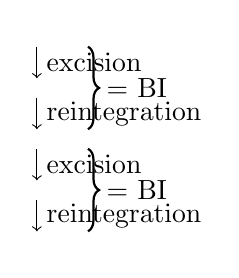
\begin{tikzpicture}[node distance=4mm]
\node (G1) {};

\node (G2) [below=of G1] {};

\node (G3) [below=of G2] {};

\node (G4) [below=of G3] {};
\node (G5) [below=of G4] {};

\draw[->] (G1) -- node[right] {excision} (G2);
\draw[->] (G2) -- node[right] {reintegration} (G3);
\draw[->] (G3) -- node[right] {excision} (G4);
\draw[->] (G4) -- node[right] {reintegration} (G5);

\node (n1) [right=of G1] {};
\node (n2) [right=of G2] {};
\node (n3) [right=of G3] {};
\node (n4) [right=of G4] {};
\node (n5) [right=of G5] {};

 \path (n3) -| node (b2) {} (n2);
    \path (n1) -| node (b1) {} (n2);
 \path (n5) -| node (b4) {} (n4);
    \path (n3) -| node (b3) {} (n4);

\draw[thick,decorate,decoration={brace, amplitude=4pt}] 
        (b1) -- (b2) node[midway, right=3pt]{
= BI

 };

    \draw[thick,decorate,decoration={brace, amplitude=4pt}] 
        (b3) -- (b4) node[midway, right=3pt]{
= BI

};
\end{tikzpicture}
\end{center}
\begin{flushright}
\scriptsize{}
\end{flushright}
\caption{A BI scenario computed by algorithm \ref{alg1}.}
\label{fig:scenarEx}
\end{figure}

\subsubsection{Conclusion}
\noindent
By expressing BI operations through the DCJ model I could show that restricting the scope of allowed DCJ operations under the constraint of performing only BI doesn't affect the 1-tandem halving distance.

This also means BI scenarios computed by the algorithm are in fact optimal DCJ scenarios and that it solves the DCJ 1-tandem halving problem for a subclass of genomes, namely genomes for which all markers must have the same orientation (sign) as their paralogs.

We will now see how to solve this problem for DCJ in the general case.

\subsection{DCJ}

\def\EP{{{\textsc{EP}}}}
\def\EC{{{\textsc{EC}}}}
\def\OC{{{\textsc{OC}}}}
\def\OP{{{\textsc{OP}}}}

In this section, because I only consider DCJ operations and no BI this time, I will drop the subscript.

 denotes the DCJ genome halving distance, towards a perfectly duplicated genome.

 denotes the DCJ 1-tandem halving distance, towards a 1-tandem duplicated genome.

~~

I recall that  can be computed using a data structure called the
\emph{natural graph}, first introduced in \cite{Mabrouk03}.  
is the graph whose vertices are the adjacencies of , and 2 vertices
are connected by an edge iff they share a paralogous \emph{extremity} (see figure
\ref{fig:NG}).

\begin{figure}
\begin{tikzpicture}[scale=1]
    \small
    \node at (9,-1) {};
    \node at (9,-2) {};
    \node at (9,-3) {};
    
    \scriptsize
    \node[draw,circle] at (0,-1) (l0) {};
    \node[draw,circle] at (1.5,-1) (l1) {};
    \node[draw,circle] at (3,-1) (l2) {};
    \node[draw,circle] at (4.5,-1) (l3) {};
    \draw (l0) -- node[above] {} (l1) -- node[above]
    {} (l2) -- node[above] {} (l3);

    \node[draw,circle] at (0,-2) (ca0) {};
    \node[draw,circle] at (2,-2) (ca1) {};
    \node[draw,circle] at (1,-3.5) (ca2) {};
    \draw (ca0) -- node[above] {} (ca1) -- node[right]
    {} (ca2) -- node[left] {} (ca0);

    \node[draw,circle] at (4,-2) (cb0) {};
    \node[draw,circle] at (6,-2) (cb1) {};
    \node[draw,circle] at (6,-3.5) (cb2) {};
    \node[draw,circle] at (4,-3.5) (cb3) {};
    \draw (cb0) -- node[above] {} (cb1) -- node [right]
    {} (cb2) -- node[below] {} (cb3) -- node [left]
    {} (cb0);

\end{tikzpicture}
\caption{The natural graph of  and the number of odd
  and even paths and cycles.}
\label{fig:NG} 
\end{figure}
As an adjacency concerns a maximum of 2 markers extremities, this graph has
a maximum degree of 2. Thus, it is composed of paths and cycles only.

Moreover, it consists of nothing but 2-cycles and 1-paths if and only
if  is a perfectly duplicated genome (a -cycle or -path is a
cycle or path containing  edges).

Using this graph, Mixtacki gave the following distance formula:
\begin{theorem}[\cite{Mixtacki08}]
Let  be a totally duplicated genome whose natural graph contains  even
cycles and  odd paths.
Then  .
\label{th:dp}
\end{theorem}
Unlike the genome halving problem, the aim of the 1-tandem halving
problem is to find a 1-tandem duplicated genome.

This induces one double-adjacency not to be reconstructed, which is
inelegant to deal with.

We will conveniently get rid of this concern.

From property \ref{prop:dtdp}, a 1-tandem genome that has been
circularized is a perfectly duplicated genome and conversely.

This allows us to establish a property that will reduce the 1-tandem
halving problem to a constraint on genome halving.

\begin{lemma}
\label{lem:unicirc=tandem}
Let  be a unilinear genome. Let  be the unicircular genome obtained by circularizing .
Then for any scenario that transforms  into a 1-tandem duplicated genome, there exists an equivalent scenario (of same length) transforming  into a unicircular perfectly duplicated genome, and vice versa.
\end{lemma}

\begin{proof}
As  and  present the same breakpoints, the scenario conversion is straightforward. It suffices to apply the same DCJ on the same breakpoints.\qed
\end{proof}

Thus, in the rest of this section, the focus will be on reconstructing
an optimal perfectly duplicated genome such that it is unichromosomal.
This is essentially a shape constraint on the genome halving
solutions.

I will follow an approach a bit similar\footnote{I had to
  expand on the ideas and add my own to make it a more complete system, due to the nature of the single tandem halving
  problem.} to what has been done in \cite{Kovac}, as
they enforced another shape constraint on optimal perfectly duplicated
genome configurations.

It consists in taking any optimal configuration then applying a number of
successive transformations (which I will call 
\emph{shapeshifting}) on it, such that they
preserve the distance, and that the optimal configuration converges
towards the desired shape.

In the following sections  will denote a totally duplicated
genome, and  its circularized version.  will be an optimal perfectly
duplicated genome for .

Following theorem \ref{th:dp}, one can observe that circularization can alter the halving distance, depending on whether the path of  is even or odd.

\begin{property}
\label{prop:dpgc}
If  is a genome such that  contains an even path, . Else, . 
\end{property}

From Mixtacki's formula (Theorem \ref{th:dp}), we know that optimal halving scenarios on circular genomes are scenarios which increase the number of even cycles at each step.
There are two ways of increasing it. Either by splitting a cycle (\textit{i.e.} extracting an even cycle from any cycle), or by merging two odd cycles.

As it can be quite complex at first sight, the shapeshifting system will first be described on a restricted class of genomes, namely those whose natural graph contains only even cycles. This way, we ensure that optimal halving scenarios consist only in cycle extractions.
This special system will then be easily generalized to all genomes by considering cycle-merging operations.

\subsubsection{Special shapeshifting}

Here we consider that  has only even cycles.
It follows that  has an even path and .

\paragraph{Anatomy of a multicircular perfectly duplicated genome.}

 is an optimal perfectly duplicated genome for .

Since  is unicircular,  contains nothing but cycles.
Therefore,  consists of circular chromosomes only.

For  to be a perfectly duplicated genome, circular chromosomes can
be of two kinds: doubled chromosomes, which can be reduced to
, and single chromosomes, which can be reduced to 
and have a \emph{paralog chromosome} in , which can be reduced to
. Thus the number of single chromosomes is even.

\paragraph{Shapeshifting.}

Any optimal perfectly duplicated genome  induces a class
 of optimal halving scenarios (the class of all optimal
DCJ scenarios transforming  into ). By observing the structure
of  and , we will look for small changes to apply to
, along two criteria:  must converge toward the
desired shape, and it must preserve its optimality.  Such small
changes are called \emph{shapeshifters}.

In our case, we want to end up with the least number of chromosomes in
 (ideally only one), therefore we will look for ways to merge
chromosomes while preserving optimality. This leads us to the
following definition:

\begin{definition}
A shapeshifter is an adjacency \aff{x}{y} such that  and  belong to \emph{different chromosomes} of  (convergence toward the desired shape), and such that \aff{x}{y} (and therefore \ass{x}{y} as well) can be reconstructed by an optimal halving scenario (preservation of optimality).
\end{definition}

For example, if  contains markers  and  in different
chromosomes,  and , and if \aff{x}{y} can be reconstructed
by an optimal halving scenario, then such scenario induces a new shape
for  such that  and  cannot be distinct chromosomes
anymore.

As for now we consider genomes whose natural graph has even cycles only, shapeshifters are adjacencies reconstructible by extracting even cycles.

\begin{property}
Adjacencies \aff{x}{y} reconstructible by extracting even cycles are those such that there exists, in , an induced subgraph which is an \emph{even} path, whose endpoints have outgoing edges  and .
\end{property}

Indeed, a DCJ reconstructing \aff{x}{y} will cut at the endpoints of such path and transform it into an even cycle.
However, it is not necessary to consider all even paths, so w.l.o.g we shall focus only on 2-paths (ie. adjancencies \aff{x}{y} that are \emph{present in }), which correspond to 2-cycles extractions.

For example,  in fig. \ref{fig:NG} is a shapeshifter, as the 2-path induced by vertices , , and  meets the requirements.

We may proceed and show how to simply apply a shapeshifter on :

Let \aff{x}{p} be the adjacency containing the extremity  in
, and \aff{q}{y} the one containing the extremity ,

it suffices to perform on  one DCJ cutting adjacencies \aff{x}{p}
and \aff{q}{y} to reconstruct \aff{x}{y} (and \aff{p}{q}), and the
equivalent DCJ on the paralogs, cutting adjacencies \ass{x}{p} and
\ass{q}{y} to reconstruct \ass{x}{y} (and \ass{p}{q}).

One can easily verify that the resulting genome is still optimal (first DCJ brings  closer to , second one reconstructs a perfectly duplicated genome). 

Now we may proceed and study the shapeshifting induced by these DCJ.

Let \aff{x}{y} be a shapeshifter in .

 and  belong to different chromosomes in , so there are only
3 possible cases depending on the types of chromosomes ( for
single chromosomes, and  for doubled ones) which contain these
markers: 1) {}, 2) {}, 3) {}. The last one could lead to different shapes. Figure
\ref{fig:shapeshift1} illustrates how the genome shape can be altered,
for each case.

\begin{figure}[htbp]
    \centering
    \begin{tabular}{ccc}
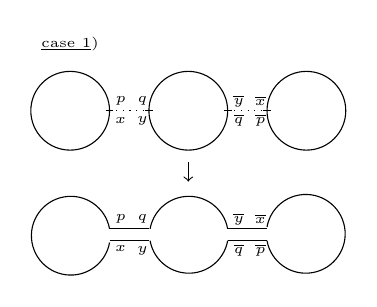
\begin{tikzpicture}[scale=0.5]
    \draw (0,0) arc (0:360:1);
    \draw (-1,0) node {};
    \draw (0,0) ++(.2,.25) node {\tiny\fst{p}};
    \draw (0,0) ++(.2,-.25) node {\tiny\fst{x}};
    \draw (0,0) ++ (-.1,0) -- ++(.2,0);

    \draw (3,0) arc (0:360:1);
    \draw (2,0) node {};
    \draw (1,0) ++(-.25,.25)  node {\tiny\fst{q}};
    \draw (1,0) ++(-.25,-.25) node {\tiny\fst{y}};
    \draw (1,0) ++ (-.1,0) -- ++(.2,0);
    \draw (3,0) ++(.2,.25)   node {\tiny\snd{y}};
    \draw (3,0) ++(.2,-.25)  node {\tiny\snd{q}};
    \draw (3,0) ++ (-.1,0) -- ++(.2,0);

    \draw (6,0) arc (0:360:1);
    \draw (5,0) node {};
    \draw (4,0) ++(-.25,.25) node {\tiny\snd{x}};
    \draw (4,0) ++(-.25,-.25) node {\tiny\snd{p}};
    \draw (4,0) ++ (-.1,0) -- ++(.2,0);

    \draw[dotted] (0,0) -- ++(1,0);
    \draw[dotted] (3,0) -- ++(1,0);

    \draw[->] (2,-1.3) -- +(0,-0.5);
    \draw(-1,1.7) node {\tiny \underline{case 1})};

    \draw (0,-3) ++(0,0) arc (10:350:1);    
    \draw (0,-3) ++(3,0) arc (10:170:1);
    \draw (0,-3) ++(3,-0.3) arc (-10:-170:1);
    \draw (0,-3) ++(4,-0.3) arc (-170:170:1);
    \draw (0,-3) ++(0,0) -- +(1,0);
    \draw (0,-3) ++(0,0) ++(.2,.25) node {\tiny\fst{p}};
    \draw (0,-3) ++(0,0) ++(.2,-.5) node {\tiny\fst{x}};
    \draw (0,-3) ++(3,0) -- +(1,0);
    \draw (0,-3) ++(1,0) ++(-.25,.25)  node {\tiny\fst{q}};
    \draw (0,-3) ++(1,0) ++(-.25,-.55) node {\tiny\fst{y}};
    \draw (0,-3) ++(3,0) ++(.2,.25)   node {\tiny\snd{y}};
    \draw (0,-3) ++(3,0) ++(.2,-.55)  node {\tiny\snd{q}};
    \draw (0,-3) ++(0,-0.3) -- +(1,0);
    \draw (0,-3) ++(4,0) ++(-.25,.25) node {\tiny\snd{x}};
    \draw (0,-3) ++(4,0) ++(-.25,-.55) node {\tiny\snd{p}};
    \draw (0,-3) ++(3,-0.3) -- +(1,0);
\end{tikzpicture}        
&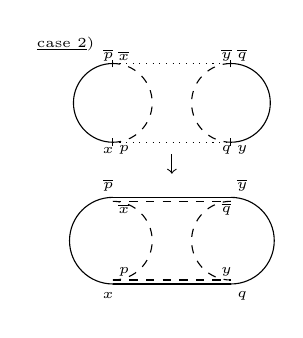
\begin{tikzpicture}[scale=0.5]
    \draw (0,2) arc (90:270:1);
    \draw[dashed] (0,0) arc (-90:90:1);
    \node at (0,1) {};
    \draw (0,2.2) ++(-.2,0) node {\tiny \snd{p}};
    \draw (0,2.2) ++(.2,0)  node {\tiny \snd{x}};
    \draw (0,-.2) ++(-.2,0) node {\tiny \fst{x}};
    \draw (0,-.2) ++(.2,0)  node {\tiny \fst{p}};
    \draw (0,1.9) -- ++(0,.2);
    \draw (0,-.1) -- ++(0,.2);

    \draw (3,0) arc (-90:90:1);
    \draw[dashed] (3,2) arc (90:270:1);
    \node at (3,1) {};
    \draw (3,2.2) ++(-.2,0) node {\tiny \snd{y}};
    \draw (3,2.2) ++(.2,0)  node {\tiny \snd{q}};
    \draw (3,-.2) ++(-.2,0) node {\tiny \fst{q}};
    \draw (3,-.2) ++(.2,0)  node {\tiny \fst{y}};
    \draw (3,1.9) -- ++(0,.2);
    \draw (3,-.1) -- ++(0,.2);

    \draw[dotted] (0,0) -- (3,0);
    \draw[dotted] (0,2) -- (3,2);

    \draw[->] (1.5,-0.3) -- +(0,-0.5);
    \draw(-1.2,2.5) node {\tiny \underline{case 2})};

    \draw (0,-3.5) ++(0,2.1) arc (90:270:1.1);
    \draw[dashed] (0,-3.5) ++(0,0) arc (-90:90:1);
    \draw (0,-3.5) ++(0,2.2) ++(-.2,0.2) node {\tiny \snd{p}};
    \draw (0,-3.5) ++(0,2.2) ++(.2,-.4)  node {\tiny \snd{x}};
    \draw (0,-3.5) ++(0,-.2) ++(-.2,-.2) node {\tiny \fst{x}};
    \draw (0,-3.5) ++(0,-.2) ++(.2,0.4)  node {\tiny \fst{p}};
    \draw (0,-3.5) ++(3,-0.1) arc (-90:90:1.1);
    \draw[dashed] (0,-3.5) ++(3,2) arc (90:270:1);
    \draw (0,-3.5) ++(3,2.2) ++(.2,0.2) node {\tiny \snd{y}};
    \draw (0,-3.5) ++(3,2.2) ++(-.2,-.4)  node {\tiny \snd{q}};
    \draw (0,-3.5) ++(3,-.2) ++(.2,-.2) node {\tiny \fst{q}};
    \draw (0,-3.5) ++(3,-.2) ++(-.2,0.4)  node {\tiny \fst{y}};
    \draw (0,-3.5) ++(0,-0.1) -- +(3,0);
    \draw (0,-3.5) ++(0,2.1) -- +(3,0);
    \draw[dashed] (0,-3.5) ++(0,0) -- +(3,0);
    \draw[dashed] (0,-3.5) ++(0,2) -- +(3,0);
\end{tikzpicture}
&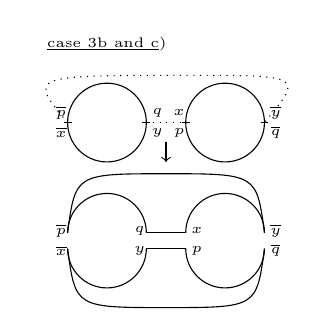
\begin{tikzpicture}[scale=0.5]
    \draw (0,0) arc (0:360:1);
    \draw (-2,0) ++(-.25,.25) node {\tiny\snd{p}};
    \draw (-2,0) ++(-.25,-.25) node {\tiny\snd{x}};
    \draw (0,0) ++ (-2.1,0) -- ++(.2,0);
    \draw (0,0) ++(.2,.25) node {\tiny\fst{q}};
    \draw (0,0) ++(.2,-.25) node {\tiny\fst{y}};
    \draw (0,0) ++ (-.1,0) -- ++(.2,0);

    \draw (3,0) arc (0:360:1);
    \draw (1,0) ++(-.25,.25)  node {\tiny\fst{x}};
    \draw (1,0) ++(-.25,-.25) node {\tiny\fst{p}};
    \draw (1,0) ++ (-.1,0) -- ++(.2,0);
    \draw (3,0) ++(.2,.25)  node {\tiny\snd{y}};
    \draw (3,0) ++(.2,-.25) node {\tiny\snd{q}};
    \draw (3,0) ++ (-.1,0) -- ++(.2,0);

    \draw[dotted] (0,0) -- ++(1,0);
    \draw[dotted] (-2,0) .. controls ++(-1,1.2) .. ++(3,1.2) .. controls
    ++(3,0) .. (3,0);

    \draw[->] (0.5,-0.5) -- +(0,-0.5);
    \draw(-1,2) node {\tiny \underline{case 3b and c})};

    \draw (0,-3) ++(0,0) ++(0,0.2) arc (0:180:1);
    \draw (0,-3) ++(3,0) ++(0,0.2) arc (0:180:1);
    \draw (0,-3) ++(0,0.2) -- +(1,0);
    \draw (0,-3) ++(-2,0.2) .. controls ++(.2,1.5) .. ++(2.5,1.5) .. controls    ++(2.3,0) .. ++(2.5,-1.5); \draw (0,-3) ++(-2,0) ++(-.25,.25) node {\tiny\snd{p}};
    \draw (0,-3) ++(-2,0) ++(-.25,-.25) node {\tiny\snd{x}};
    \draw (0,-3) ++(0,0) ++(-.25,.25) node {\tiny\fst{q}};
    \draw (0,-3) ++(0,0) ++(-.25,-.25) node {\tiny\fst{y}};
    \draw (0,-3) ++(0,0) ++(0,-.2) arc (0:-180:1);
    \draw (0,-3) ++(3,0) ++(0,-.2) arc (0:-180:1);
    \draw (0,-3) ++(0,-0.2) -- +(1,0);
    \draw (0,-3) ++(-2,-0.2) .. controls ++(.2,-1.5) .. ++(2.5,-1.5) .. controls    ++(2.3,0) .. ++(2.5,1.5); \draw (0,-3) ++(1,0) ++(.2,.25)  node {\tiny\fst{x}};
    \draw (0,-3) ++(1,0) ++(.2,-.25) node {\tiny\fst{p}};
    \draw (0,-3) ++(3,0) ++(.2,.25)  node {\tiny\snd{y}};
    \draw (0,-3) ++(3,0) ++(.2,-.25) node {\tiny\snd{q}};
\end{tikzpicture}
\end{tabular}
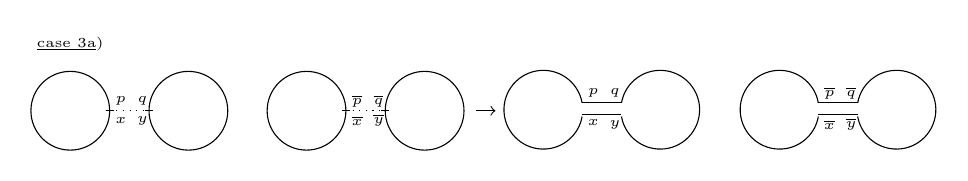
\begin{tikzpicture}[scale=0.5]
    \draw (0,0) arc (0:360:1);
    \draw (-1,0) node {};
    \draw (0,0) ++(.2,.25) node {\tiny\fst{p}};
    \draw (0,0) ++(.2,-.25) node {\tiny\fst{x}};
    \draw (0,0) ++ (-.1,0) -- ++(.2,0);

    \draw (3,0) arc (0:360:1);
    \draw (2,0) node {};
    \draw (1,0) ++(-.25,.25)  node {\tiny\fst{q}};
    \draw (1,0) ++(-.25,-.25) node {\tiny\fst{y}};
    \draw (1,0) ++ (-.1,0) -- ++(.2,0);

    \draw[dotted] (0,0) -- ++(1,0);

    \draw (6,0) arc (0:360:1);
    \draw (5,0) node {};
    \draw (6,0) ++(.2,.25) node {\tiny\snd{p}};
    \draw (6,0) ++(.2,-.25) node {\tiny\snd{x}};
    \draw (6,0) ++ (-.1,0) -- ++(.2,0);

    \draw (9,0) arc (0:360:1);
    \draw (8,0) node {};
    \draw (7,0) ++(-.25,.25)  node {\tiny\snd{q}};
    \draw (7,0) ++(-.25,-.25) node {\tiny\snd{y}};
    \draw (7,0) ++ (-.1,0) -- ++(.2,0);

    \draw[dotted] (6,0) -- ++(1,0);

\draw[->] (9.3,0) -- +(0.5,0);
\draw(-1,1.7) node {\tiny \underline{case 3a})};

    \draw (12,0.2) ++(0,0) arc (10:350:1);
    \draw (12,0.2) ++(1,0) arc (170:-170:1);
    \draw (12,0.2) ++(0,0) -- +(1,0);
    \draw (12,0.2) ++(0,0) ++(.2,.25) node {\tiny\fst{p}};
    \draw (12,0.2) ++(0,0) ++(.2,-.5) node {\tiny\fst{x}};
    \draw (12,0.2) ++(0,-0.3) -- +(1,0);
    \draw (12,0.2) ++(1,0) ++(-.25,.25)  node {\tiny\fst{q}};
    \draw (12,0.2) ++(1,0) ++(-.25,-.55) node {\tiny\fst{y}};
    \draw (12,0.2) ++(6,0) arc (10:350:1);
    \draw (12,0.2) ++(7,0) arc (170:-170:1);
    \draw (12,0.2) ++(6,0) -- +(1,0);
    \draw (12,0.2) ++(6,-0.3) -- +(1,0);
    \draw (12,0.2) ++(6,0) ++(.2,.25)   node {\tiny\snd{p}};
    \draw (12,0.2) ++(6,0) ++(.2,-.55)  node {\tiny\snd{x}};
    \draw (12,0.2) ++(7,0) ++(-.25,.25) node {\tiny\snd{q}};
    \draw (12,0.2) ++(7,0) ++(-.25,-.55) node {\tiny\snd{y}};
\end{tikzpicture}
    \caption{The different shapes that can be obtained by applying a shapeshifter.}
    \label{fig:shapeshift1}
\end{figure}

More formally, one can represent shapeshifting as a system of rewriting rules:
\begin{center}
    \begin{tabular}{ll@{}ll@{}ll}
        1) & {}   & 3.a) & {} & 3.c) & {} \\
        2) & {} & 3.b) & {} \\
    \end{tabular}
\end{center}

This is convenient as one can deduce useful properties by looking at these rules, which we are about to do, in order to study limit states of the system.

\begin{property}
\label{prop:decreasing}
 Shapeshifting cannot increase the number of chromosomes.
\end{property}

Thus, any limit-cycle necessarily uses rules that do not change the number of chromosomes. Moreover, using rule 2 would eventually lead to using rule 3.b or 3.c as doubled chromosomes are changed into single chromosomes.

\begin{property}
\label{prop:limitcycle}
Any limit-cycle of the system necessarily uses rule 3.b or 3.c.
\end{property}

\begin{property}
\label{prop:invariant}
  Parity of  is invariant by shapeshifting.
\end{property}

\begin{property}
\label{prop:steadystate}
 A unicircular genome (ie. one doubled chromosome) is the only steady state of the system.
\end{property}

\begin{lemma}
\label{lem:under3}
  By shapeshifting, the number of chromosomes in  can always be decreased under 3.
\end{lemma}

\begin{proof}
Having 3 chromosomes or more guarantees existence of shapeshifters decreasing their number.
Consider the case where  contains only 2 single chromosomes  and . Label the markers from  by the chromosome which holds them in . Adding new chromosomes necessarily creates shapeshifters between at least one of the new chromosomes and  or . Such shapeshifter decreases the number of chromosomes.\qed
\end{proof}

\begin{lemma}
\label{lem:oddCd}
There exists a unicircular optimal perfectly duplicated genome for  if and only if  has an \emph{odd} number of doubled chromosomes.
\end{lemma}
\begin{proof}
Straightforward from lemma \ref{lem:under3} and property \ref{prop:invariant}.\qed
\end{proof}

\begin{lemma}
\label{lem:evenCd}
If  has an \emph{even} number of doubled chromosomes, the minimum number of DCJ operations required to reconstruct a unicircular perfectly duplicated genome is , and it can always be attained.
\end{lemma}
\begin{proof}
From lemma \ref{lem:oddCd}, it is impossible to attain a unicircular genome in  operations. However, from lemma \ref{lem:under3} and property \ref{prop:limitcycle}, it is then always possible to attain two single chromosomes.

Two single chromosomes can then be transformed into one doubled chromosome by one DCJ.\qed
\end{proof}

In conclusion, special shapeshifting allows to compute the tandem distance of any genome  such that  contains only even cycles.
 \begin{theorem}
\label{th:restricted}
Let  be a totally duplicated genome such that  contains only even cycles.
Let  be its circularized version, and  any optimal perfectly duplicated genome for .

 if and only if  contains an odd number of doubled chromosomes. Else .
\end{theorem}

\begin{proof} 
Since  contains only even cycles, it contains an even path. Therefore from property \ref{prop:dpgc}, .

From lemma \ref{lem:unicirc=tandem} we have that  if and only if there exists a unicircular optimal perfectly duplicated genome.
Theorem then follows from lemmas \ref{lem:oddCd} and \ref{lem:evenCd}.\qed 
\end{proof}

The next step is to generalize the shapeshifting system in order to take all possible genomes into account.

\subsubsection{General shapeshifting}

As usual,  is a totally duplicated genome,  its circularized version, and  an optimal perfectly duplicated genome for .
I will also keep the same notations related to shapeshifters as in the previous section: \aff{x}{y} is a shapeshifter such that  (resp. ) is present in chromosome  (resp. ) of , through adjacency \aff{x}{p} (resp. \aff{q}{y} ).

The difference with special shapeshifting is that, \emph{in addition} to everything covered by special shapeshifting, optimal halving scenarios may now also contain cycle merges. Therefore I have to consider shapeshifters that are adjacencies which can be optimally reconstructed through merges.

\begin{property}
Adjacencies \aff{x}{y} reconstructible by merges are those such that extremities  and  are in \emph{two distinct odd cycles} of .
\end{property}

Corresponding shapeshifters can still allow the same shapeshifting rules depending on the types of  and . Additionally, it is now possible to have  and .

This implies that  and induces yet another
degenerated case.

The general shapeshifting set of rule becomes: 
\begin{center}
    \begin{tabular}{ll@{}ll@{}ll}
        1) & {}   & 3.a) & {} & 3.c) & {} \\
        2) & {} & 3.b) & {} & \textbf{3.d)} & {} \\
    \end{tabular}
\end{center}
This new rule gives general shapeshifting a very interesting property.

\begin{property}
Rule 3.d changes parity of .
\end{property}

\begin{lemma}
\label{lem:parity}
If  contains odd cycles, and if  is made of two single chromosomes, then rule 3.d can be applied.
\end{lemma}
\begin{proof}
As  contains odd cycles, there are merges in any optimal scenario from  to . Thus, there exists an adjacency \aff{x}{p} in  such that the adjacencies concerning extremities  and  are in two distinct odd cycles of . By definition, the adjacency concerning extremity  is in the same cycle as the one concerning .
Therefore, \afs{x}{p} is a shapeshifter inducing rule 3.d.\qed
\end{proof}
\begin{corollary}
Presence of odd cycles in  ensures a unicircular optimal
perfectly duplicated genome that can always be reached, as rule 3.d can always adjust the parity of  if needed. \end{corollary}

\begin{theorem}
\label{th:generalized}
Let  be a totally duplicated genome such that  contains at least one odd cycle, and  its circularized version.

Then .
\end{theorem}

\begin{proof} 
    From lemma \ref{lem:unicirc=tandem} we have  iff there exists a unicircular optimal perfectly
    duplicated genome.  Corollary from lemma \ref{lem:parity} ensures
    that there does.\looseness=-1 \qed
\end{proof}

\subsubsection{Distance}

I may finally state a definite formula for the 1-tandem halving distance, as well as results on computational complexity of this problem, by gathering results from the previous sections.

\begin{theorem}



Where  is a parameter that is equal to 1 iff  is even and , and is equal to 0 otherwise. ,  and  are respectively the number of even cycles, even paths and odd cycles in .

\end{theorem}

\begin{proof} 
Straightforward from theorems \ref{th:restricted} and \ref{th:generalized}.\qed 
\end{proof}

\begin{theorem}
  can be computed in linear time.
\end{theorem}
\begin{proof}
 can be computed in linear time, as well as an optimal perfectly duplicated genome.\qed
\end{proof}

\begin{theorem}
    Computing a scenario can be done in quadratic time.
\end{theorem}
\begin{proof}
An optimal perfectly duplicated genome can be computed in  time using Mixtacki's algorithm (\cite{Mixtacki08}).
From lemma \ref{lem:under3}, one can reduce  to the minimum number of chromosomes using  shapeshifters. Each shapeshifter can be found in  time, so we have a  time shapeshifting algorithm.
An optimal DCJ scenario between  and  can then be computed in  time using Yancopoulos' algorithm (\cite{Yancopoulos05}). Thus the algorithm takes quadratic time on the whole.\qed
\end{proof}

\subsection{Closing words and credits}

I was asked by Jean-Stéphane Varré to work on tandem duplications for my master's degree in 2010. I developed the single tandem halving problem as a starting point.

~~

\textbf{On halving by block interchange}

~~

Aida Ouangraoua taught me Anne Bergeron's method for sorting by DCJ as in \cite{BMS06}.

Aida O. also heavily insisted I use her alternate\footnote{non-working} proof for the distance formula. She then rephrased one of my intermediate proofs (proof \ref{proof:proofType2}).

Jean-Stéphane V. drew some of the figures for the article.

I developed my BI 1-tandem halving study mainly with inspiration from \cite{Mixtacki08}. I will add I have been very admirative of Julia Mixtacki's work, in this paper and in the others, for it always presented results with very elegant proofs and reasonings. Her style has been and remains a major inspiration for me.

~

\textbf{On halving by DCJ}

~~

Jean-Stéphane V. drew some of the figures.

I developed shapeshifting with inspiration from \cite{Kovac}. I would like to thank the authors of that paper as it allowed me to gain a much better insight into the space of genome halving scenarios.

Aida O. did not contribute as she was in Canada during most of the time I have been working on this. She participated in some of the early discussions, before shapeshifting was developed.

Once again I took care of proving every single result from these papers.

\section{Model III: Partial tandem duplication}
\label{sec:partialdup}

This work has been published in \cite{Thomas12}. 

Along with the single tandem halving by DCJ, I studied other tandem models:

I studied a model where only a subset of the markers are duplicated. I could not settle complexity of this problem but provided a heuristic algorithm.

I also designed and studied various extended models were multiple tandem duplications occurred such that markers could be present in more than 2 copies.

I proved NP-hardness of all these variants.

\subsection{Model}

\subsubsection{Considered genomes}

I use duplicated genomes, perfectly duplicated genomes as defined in section \ref{sec:notations2}, and dedoubled genomes as defined in section \ref{sec:dedouble}.

I also introduce a generalization of tandem duplicated genomes, namely \emph{k-tandem duplicated genomes}.

\begin{definition}
A \emph{k-tandem duplicated genome} is a totally duplicated genome which can
be reduced to a unilinear dedoubled genome consisting of  distinct markers.
\end{definition}

For example, the genome
 is a 2-tandem
duplicated genome that can be reduced to the dedoubled genome 

.

Naturally, this new definition is consistent with the previous definition of a 1-tandem duplicated genome.

\subsubsection{Considered operations}

The considered operation model is the DCJ model.

\subsection{Disrupted Single Tandem Halving}
\label{sec:disrupted}

As we could solve the 1-tandem halving problem, a first direction for generalization will be considering genomes containing both duplicated and non-duplicated markers, as it is in better accordance with real biological data.

This can be seen as a 1-tandem halving problem in which adjacencies between duplicated markers can be broken by presence of non-duplicated ones. In other words, non-duplicated markers \emph{disrupt} the 1-tandem halving.

\begin{definition}
The \emph{disrupted 1-tandem halving problem} is a variant of the 1-tandem halving problem in which the genome contains both duplicated and non-duplicated markers. The duplicated markers have to be regrouped and arranged in tandem. The corresponding distance, the \emph{disrupted 1-tandem halving distance}, is denoted .
\end{definition}

\subsection{DCJ}

Although a polynomial solution could not be found, in this section I describe a polynomial approximate algorithm and precise its bounds.

I suspect this problem to be NP-hard due to its relation to k-tandem halving.

\subsubsection{Preliminary analysis.}

Any optimal disrupted 1-tandem halving scenario performs two tasks: it gathers duplicated markers together (gathering phase), and it reorganizes them in a tandem (tandem phase).

\begin{definition}
A \emph{break} is an interval of non-duplicated markers surrounded by duplicated markers.
\end{definition}

From now on,  is a duplicated genome containing  duplicated markers separated by  breaks.

\begin{definition}
A \emph{gathering operation} is a DCJ which reduces the number of breaks in .
\end{definition}

Note that the presence of excisions in the gathering phase may produce a genome consisting of multiple chromosomes.

Excisions and their resulting chromosomes will be categorized depending on whether said chromosomes can be reintegrated at best in their source chromosome while increasing the number of even cycles (\emph{good} excision/chromosome), leaving it unchanged (\emph{neutral}) or decreasing it (\emph{bad}).

As this variation in  changes the tandem distance, we get the following property.
\begin{property}
Once the gathering phase is over in , the remaining distance is , with  the number of neutral chromosomes and  the number of bad ones.
\end{property}

The key to build an optimal disrupted 1-tandem halving scenario is to find a gathering scenario that maximizes the number of even cycles while minimizing the number of neutral and bad excisions.

\subsubsection{Optimizing the gathering scenario.}

A DCJ can decrease the number of breaks by at most 1.

\begin{property}
The minimum number of gathering operations is .
\end{property}

Gathering operations are DCJ whose breakpoints are on path endpoints from . Breakpoints in two distinct paths will merge them, while breakpoints on the endpoints of a same path will circularize it.

\begin{property}
An optimal gathering operation is one that either merges two odd paths, or circularizes an even path.
\end{property}

I now give the maximum number of even cycles a set of  gathering operations can create.

\begin{lemma}
A shortest gathering scenario can create up to  even cycles.
\end{lemma}
\begin{proof}
sketch of proof: Any even path can be circularized by one DCJ, while any two odd paths can be turned into two even cycles with 2 DCJs. Since  breaks induce  paths in , the number of gathering operations we can use is .\qed
\end{proof}

\begin{corollary}
\label{cor:lb}
.
\end{corollary}

This is assuming a shortest gathering phase produced no bad nor neutral chromosome, and that we are in the best case for the remaining tandem distance ().

Neutral excisions induce a penalty which is the same as performing a
non-optimal gathering reversal, bad excisions are even
worse. Thus the greedy heuristic will proceed as follows: Look
for an optimal gathering operation which is a reversal or a good
excision. When there is none, perform a non-optimal gathering
reversal. \looseness=-1

Let  be the number of even cycles produced by the heuristic, then we obtain the following upperbound: .

In the worst case,  can be equal to 0, however, the algorithm
seems to perform pretty well on random genomes, giving values close to the lowerbound.

\subsection{Beyond duplications: Multiple tandem halving}
\label{sec:mth}

Unlike 1-tandem halving, k-tandem halving can be defined in various
ways (is the content of each tandem fixed or only the number? Is the order constrained? etc...). I explored various cases, each time describing a more constrained model:

\begin{itemize}
\item Fixing the number of tandem to be reconstructed (), the problem is NP-hard. 

\item Fixing the markers to be contained in each of the  tandem, the problem remains NP-hard.

\item Fixing the order in which the tandem appear in the ancestral genome, still NP-hard. 

\item Lastly, a \emph{signed} version where the relative orientation of the
tandems is fixed is also NP-hard. 
\end{itemize}

It is unfortunate, as multiple tandems are more relevant from a biological point of view.

Detailed study and proofs follow.

\subsubsection{Genome Dedoubling}

As k-tandem duplicated genomes can be reduced to dedoubled
genomes, I will restate the \emph{genome dedoubling problem} (already studied in section \ref{sec:dedoubling}).

\begin{definition}
Given a rearranged duplicated genome  composed of a single chromosome, the
\emph{genome dedoubling problem} consists in finding a dedoubled genome  such
that the distance between  and  is minimal.
\end{definition}

I recall the general working of an optimal genome dedoubling algorithm, using  (refer to \ref{sec:dedoubling} for definition of  as well as detailed proofs):

\begin{enumerate}
\item{Pick a maximum number of pairwise disjoint cycles in .}

\item{Split them all into 1-cycles.}

\item{Extract 1-cycles concerning other markers in any way until you obtain at least  disjoint 1-cycles.}

\item{\textit{(unilinear variant only)} merge all remaining cycles with the path of .}

\end{enumerate}

I remind the reader the genome dedoubling problem is NP-hard, since picking a maximum number of pairwise disjoint cycles in  is NP-hard. 

Naturally the unilinear variant is NP-hard as well.

I state a similar result for a small variation on this problem as it will prove useful later.

\begin{definition}
A \emph{loosely dedoubled genome} is a unilinear totally duplicated genome  such that for each marker , either \afs{x}{x}, \afs{-x}{x}, \aff{x}{\msnd{x}} or \aff{-x}{\msnd{x}} is an adjacency of .
\end{definition}

Essentially it is a unilinear dedoubled genome in which the sign of each marker is disregarded. It means that for each marker ,  either has one 1-cycle for  and one edge for  in the path, or 2 consecutive edges for  in the path.

\begin{definition}
The \emph{loose dedoubling problem} is a variant of the genome dedoubling problem where the aim is a loosely dedoubled genome. 
\end{definition}

\begin{theorem}
The loose genome dedoubling problem is NP-hard.
\end{theorem}
\begin{proof}
The loose variant allows one to avoid having to extract 1-cycles from the path when it presents consecutive edges for a same marker. However, in order to attain the minimum number of operation, it is still required to minimize the number of cycles to be merged with the path. In other words, one still has to pick a maximum number of pairwise disjoint cycles in .\qed
\end{proof}

We may now proceed and study k-tandem halving problems.

\subsubsection{Fixed tandem number}

Here we just aim at reconstructing k tandems, regardless of their respective marker contents.

\begin{definition}
    Let  be a totally duplicated genome consisting of  distinct markers, let  be an
    integer. The \emph{-tandem halving} problem consists in finding
    a -tandem duplicated genome  such that the distance between
     and  is minimal.
\end{definition}

\begin{theorem}
The -tandem halving problem is NP-hard.
\end{theorem}

\begin{proof}
Genome Dedoubling problem is the particular case of k-tandem halving where  = . \qed
\end{proof}

\subsubsection{Fixed tandem content}

The goal is now to reconstruct k tandems whose respective marker contents are given.

\begin{definition}
    Let  be a totally duplicated genome, consisting of  distinct markers, let  be a partition of the set of distinct markers.
The \emph{-fixed-tandem halving} problem consists in finding a -tandem duplicated genome  such that each
    tandem is made of the markers of a  set, and such that the distance between  and  is minimal.
\end{definition}

\begin{theorem}
The -fixed-tandem halving problem is NP-hard.
\end{theorem}

\begin{proof}
    Genome Dedoubling problem is the particular case of
    -fixed-tandem problem where P is a set of singleton sets. \qed
\end{proof}

\subsubsection{Fixed tandem content and fixed tandem order}

I will now constrain, additionally to the tandems content, the order in which
the tandems are appearing in the final configuration.

\begin{definition}
    Let  be a totally duplicated genome, consisting of  distinct markers, let  be a partition of the set of distinct markers.
The \emph{-ordered-tandem halving} problem consists in finding a -tandem duplicated genome  such that consecutive tandems are made of the markers of consecutives  sets, and such that the distance between  and  is minimal.
\end{definition}

This is a very strong contraint, however the problem is
still NP-hard.
Let's first consider the genome dedoubling variant of this problem (ie. the case where P is a set of singleton sets).

\begin{theorem}
Ordered genome dedoubling problem is NP-hard.
\end{theorem}
\begin{proof}
Constraining the markers order in a dedoubled genome is a constraint on the path of . Thus, the choice of pairwise disjoint cycles remains.\qed
\end{proof}
\begin{corollary}
The -ordered-tandem halving problem is NP-hard.
\end{corollary}

\subsubsection{Signed k-tandem halving} 

I will now enforce a constraint which makes genome dedoubling polynomial, and see if it can lead to a polynomial k-tandem halving problem.

\begin{definition}
The \emph{signed dedoubling problem} is a variant of the genome dedoubling problem where the sign of each doublet (ie. \afs{x}{x} or \aff{-x}{\msnd{x}}) is fixed. 
\end{definition}

\begin{lemma}
The signed dedoubling problem is polynomial.
\end{lemma}
\begin{proof}
There is no more possible choice of pairwise disjoint cycles. Indeed, the sign constraint enforces a particular edge (and thus a particular cycle) to be picked.\qed
\end{proof}

I will now conduct a deeper analysis of the signed k-tandem halving problem.

\paragraph*{Genome defragmentation}

 Similarly to the disrupted 1-tandem-halving problem, marker subsets have to be grouped during an optimal scenario. The main difference is that there are several groups to be reconstructed, disrupting each other. Thus, \emph{defragmentation} seems to be a more appropriate term.

\begin{definition}
A \emph{fragment} is an interval of markers from a same group, surrounded by markers from others groups \emph{or telomeres}.
\end{definition}

\begin{definition}
A \emph{defragmentation operation} is a DCJ which reduces the number of fragments in .
\end{definition}

\begin{lemma}
\label{lem:defrag}
Computing the minimum number of defragmentation operations is NP-hard.
\end{lemma}
\begin{proof}
Any loose dedoubling problem instance can be seen as a defragmentation problem under the constraint that each group is split in no more than 2 fragments (one marker stands for a fragment in a genome).\qed 

\end{proof}

\begin{theorem}
Signed k-tandem halving problem is NP-hard.
\end{theorem}

\begin{proof}
This is proven by reduction, from the problem of computing the minimum number of defragmentation operations, to a subclass of signed k-tandem halving.
Consider the class of genomes for which there exists an optimal scenario consisting only of a defragmentation phase. Theorem then follows from lemma \ref{lem:defrag}.\qed
\end{proof}

\subsection{Closing words and credits}

~

\textbf{On disrupted tandem halving}

I recall I originally developed the single tandem halving problem as a starting point for disrupted tandem halving.

Jean-Stéphane V. drew some of the figures for the article.

\textbf{On multiple tandem halving}

I developed, studied and proved all of these variants alone.

Again, Aida O. did not participate as she was in Canada while I worked on this paper.

As usual I took care of proving every single result from this paper. 

\section{Conclusion}

To conclude this section, here is a table containing all of my results.

\begin{center} 
\resizebox{16cm}{!}{
    \begin{tabular}{|c||c|c|} 
       \hline
 Problem & Input genome & Goal configuration \\
        \hline
Genome Dedoubling & Totally duplicated & Dedoubled \\
        1-tandem Halving     &  Totally duplicated  &  1-tandem  \\
k-tandem Halving & Totally duplicated & k tandems \\ 
disrupted 1-tandem Halving & Duplicated & Tandem\\

\hline
    \end{tabular}
}\end{center}

\begin{center} 

\resizebox{16cm}{!}{
    \begin{tabular}{|c|c||c|} 
       \hline
 Problem & Operation model &  Complexity \\
        \hline
Genome Dedoubling & DCJ or Reversal & NP-hard (FPT in the number of cycles) \\
        1-tandem Halving     &  DCJ or Block Interchange   &   (scenario in )\\
k-tandem Halving & DCJ & NP-hard \\ 
disrupted 1-tandem Halving & DCJ &  open \\

\hline
    \end{tabular}
}\end{center}

\part*{General conclusion}

I think my PhD thesis could be summarized by the following sentence:

~

\textit{``Biological reality is NP-hard, polynomial problems come with a catch: they don't make much sense".}

~

The catch being no duplicated content, or an exponential number of different genomes that are all optimal, or other aspects causing awkward moments in bioinformatics conferences when biologists ask questions.

From a computer science and mathematical point of view, however, it's much more interesting.

We've seen that data structures are a powerful tool to shift focus.

On this matter I'll add that any algorithm can be seen as a data structure itself, and this allows a certain freedom in splitting complexity : for example in some cases an   time algorithm could be implemented as a loop of  steps each using a structure built in , or a loop of  steps using a linear structure instead... this kind of reasoning is what allowed me to find the ``magic" property (``the smallest overlapping interval is an optimal operation") for single-tandem halving by block interchange.

I'll conclude by saying that this work on the whole is meant to be seen as a starting point in the study of alternate explanative models for the presence of replicated markers. As said models are taken directly from biological studies, they are obviously not new. However, it is the first time they are studied in the context of classical rearrangement problems.

While most people would notice the diversity in mathematical proofs throughout my papers, I find it is even more stimulating to try to grasp the subtle underlying similarities they must share, since down the line they really are the expression of different analyses for similar problems.

Obvious further perspectives would be the study of other duplication hypotheses, or combination of previously studied ones, even though I feel the mastery of previously studied models and their behavior towards multiple operation models should take priority.

For example, the attempt at solving genome dedoubling by reversal with unoriented genomes (cf. section \ref{unoriented}) was never published and the reason is that the answer we seemed to find (computing an optimal reversal scenario through dynamic programming, in polynomial time) was not a satisfying one. My real goal with this work was to be able to directly compute the orientation cost without the need for building an optimal scenario, just as it was done for classical sorting by reversal in \cite{BMS-04}. I find this kind of result allows a much deeper understanding of the studied problem.

In the same line of thought, I'd consider that even the classical genome halving by reversal, as solved in \cite{Mabrouk98}, doesn't provide a satisfying answer and would deserve further studies.

More generally, I think that while operational research provides very interesting concepts to tackle hard problems, it should be reserved, as intended, to hard problems, be it NP-hard rearrangement problems or software application meant to process very large genomes. In the context of theoretical papers, finding a polynomial answer through such techniques should be seen as an encouragement to find a more elegant method that would provide a better understanding of the problem.

Finally, to give a few words about where I see this field going in a couple years, I would say that unless major changes occur, I do not foresee a bright future in rearrangements for the LIFL, given the type of people working in bioinformatics there.

Even though I wish them success in the name of scientific progress, I don't think it can be done by blatantly trashing ethics, claiming ownership of other people's work by nothing more than writing their names at the highest possible place on the paper, somewhat reminiscent of the way a dog would leave its mark on a fire hydrant.

\begin{thebibliography}{}

\bibitem[Alekseyev and Pevzner, 2007]{AP07}
Alekseyev, M.~A. and Pevzner, P.~A. (2007).
\newblock Whole genome duplications, multi-break rearrangements, and genome
  halving problem.
\newblock In {\em Proceedings of the eighteenth annual ACM-SIAM symposium on
  Discrete algorithms}, pages 665--679. Society for Industrial and Applied
  Mathematics.

\bibitem[Alekseyev and Pevzner, 2008]{A08}
Alekseyev, M.~A. and Pevzner, P.~A. (2008).
\newblock Multi-break rearrangements and chromosomal evolution.
\newblock {\em Theoretical Computer Science}, 395(2):193--202.

\bibitem[Angibaud et~al., 2007]{A07}
Angibaud, S., Fertin, G., Rusu, I., Th{\'e}venin, A., and Vialette, S. (2007).
\newblock A pseudo-boolean programming approach for computing the breakpoint
  distance between two genomes with duplicate genes.
\newblock In {\em Comparative Genomics}, pages 16--29. Springer.

\bibitem[Bader et~al., 2001]{BMY01}
Bader, D.~A., Moret, B. M.~E., and Yan, M. (2001).
\newblock A linear-time algorithm for computing inversion distance between
  signed permutations with an experimental study.
\newblock {\em Journal of Computational Biology}, 8:483--491.

\bibitem[Bafna and Pevzner, 1998]{BP98}
Bafna, V. and Pevzner, P. (1998).
\newblock Sorting by transpositions.
\newblock {\em SIAM Journal on Discrete Mathematics}.

\bibitem[Bafna and Pevzner, 1995]{BP95}
Bafna, V. and Pevzner, P.~A. (1995).
\newblock Sorting permutations by transpositions.
\newblock In Clarkson, K.~L., editor, {\em SODA}, pages 614--623. ACM/SIAM.

\bibitem[Bailey et~al., 2004]{B04}
Bailey, J., Baertsch, R., Kent, W., Haussler, D., and Eichler, E. (2004).
\newblock Hotspots of mammalian chromosomal evolution.
\newblock {\em Genome Biology}, 5(4):R23.

\bibitem[B{\'e}rard et~al., 2007]{BBCP07}
B{\'e}rard, S., Bergeron, A., Chauve, C., and Paul, C. (2007).
\newblock Perfect sorting by reversals is not always difficult.
\newblock {\em Computational Biology and Bioinformatics, IEEE/ACM Transactions
  on}, 4(1):4--16.

\bibitem[B{\'e}rard et~al., 2008]{BBCP08}
B{\'e}rard, S., Chauve, C., and Paul, C. (2008).
\newblock A more efficient algorithm for perfect sorting by reversals.
\newblock {\em Information processing letters}, 106(3):90--95.

\bibitem[B{\'e}rard et~al., 2012]{SCJ1}
B{\'e}rard, S., Gallien, C., Boussau, B., Sz{\"o}ll{\H{o}}si, G.~J., Daubin,
  V., and Tannier, E. (2012).
\newblock Evolution of gene neighborhoods within reconciled phylogenies.
\newblock {\em Bioinformatics}, 28(18):i382--i388.

\bibitem[Bergeron, 2001]{B01}
Bergeron, A. (2001).
\newblock A very elementary presentation of the hannenhalli-pevzner theory.
\newblock {\em Lecture Notes in Computer Science}, 2089:106--117.

\bibitem[Bergeron, 2005]{B-05}
Bergeron, A. (2005).
\newblock A very elementary presentation of the hannenhalli-pevzner theory.
\newblock {\em Discrete Applied Mathematics}, 146(2):134--145.

\bibitem[Bergeron et~al., 2004]{BMS-04}
Bergeron, A., Mixtacki, J., and Stoye, J. (2004).
\newblock Reversal distance without hurdles and fortresses.
\newblock In {\em In proc. of Combinatorial Pattern Matching. LNCS 3109}, pages
  388--399. Springer-Verlag.

\bibitem[Bergeron et~al., 2005]{BMS05}
Bergeron, A., Mixtacki, J., and Stoye, J. (2005).
\newblock On sorting by translocations.
\newblock In Miyano, S., Mesirov, J., Kasif, S., Istrail, S., Pevzner, P., and
  Waterman, M., editors, {\em Research in Computational Molecular Biology},
  volume 3500 of {\em Lecture Notes in Computer Science}, pages 615--629.
  Springer Berlin Heidelberg.

\bibitem[Bergeron et~al., 2006]{BMS06}
Bergeron, A., Mixtacki, J., and Stoye, J. (2006).
\newblock A unifying view of genome rearrangements.
\newblock In Bücher, P. and Moret, B., editors, {\em Algorithms in
  Bioinformatics}, volume 4175 of {\em Lecture Notes in Computer Science},
  pages 163--173. Springer Berlin Heidelberg.

\bibitem[Bergeron et~al., 2008]{BMS08}
Bergeron, A., Mixtacki, J., and Stoye, J. (2008).
\newblock Hp distance via double cut and join distance.
\newblock In {\em Combinatorial Pattern Matching}, pages 56--68. Springer.

\bibitem[Berman and Fujito, 1995]{BF-95}
Berman, P. and Fujito, T. (1995).
\newblock Approximating independent sets in degree 3 graphs.
\newblock In {\em In proc. of Workshop on Algorithms and Data Structures. LNCS
  955}, pages 449--460. Springer-Verlag.

\bibitem[Biller et~al., 2013]{BFM13}
Biller, P., Feij{\~a}o, P., and Meidanis, J. (2013).
\newblock Rearrangement-based phylogeny using the single-cut-or-join operation.
\newblock {\em IEEE/ACM Transactions on Computational Biology and
  Bioinformatics (TCBB)}, 10(1):122--134.

\bibitem[Blin et~al., 2007]{BCFRV07}
Blin, G., Chauve, C., Fertin, G., Rizzi, R., and Vialette, S. (2007).
\newblock Comparing genomes with duplications: a computational complexity point
  of view.
\newblock {\em IEEE/ACM Transactions on Computational Biology and
  Bioinformatics (TCBB)}, 4(4):523--534.

\bibitem[Blin et~al., 2004]{BFC04}
Blin, G., Fertin, G., Chauve, C., et~al. (2004).
\newblock The breakpoint distance for signed sequences.
\newblock In {\em 1st Conference on Algorithms and Computational Methods for
  biochemical and Evolutionary Networks (CompBioNets' 04)}, volume~3, pages
  3--16.

\bibitem[Blin et~al., 2009]{BFSV09}
Blin, G., Fertin, G., Sikora, F., and Vialette, S. (2009).
\newblock The exemplar breakpoint distance for non-trivial genomes cannot be
  approximated.
\newblock In {\em WALCOM: Algorithms and Computation}, pages 357--368.
  Springer.

\bibitem[Braga et~al., 2010]{BWS10}
Braga, M., Willing, E., and Stoye, J. (2010).
\newblock Genomic distance with dcj and indels.
\newblock In Moulton, V. and Singh, M., editors, {\em Algorithms in
  Bioinformatics}, volume 6293 of {\em Lecture Notes in Computer Science},
  pages 90--101. Springer Berlin Heidelberg.

\bibitem[Braga, 2009]{B09}
Braga, M.~D. (2009).
\newblock baobabluna: the solution space of sorting by reversals.
\newblock {\em Bioinformatics}, 25(14):1833--1835.

\bibitem[Braga et~al., 2007]{BS07}
Braga, M.~D., Sagot, M.-F., Scornavacca, C., and Tannier, E. (2007).
\newblock The solution space of sorting by reversals.
\newblock In {\em Bioinformatics Research and Applications}, pages 293--304.
  Springer.

\bibitem[Braga and Stoye, 2010]{BS10}
Braga, M.~D. and Stoye, J. (2010).
\newblock The solution space of sorting by dcj.
\newblock {\em Journal of Computational Biology}, 17(9):1145--1165.

\bibitem[Braga and Stoye, 2013]{Br13}
Braga, M.~D. and Stoye, J. (2013).
\newblock Restricted dcj-indel model revisited.
\newblock In {\em Advances in Bioinformatics and Computational Biology}, pages
  36--46. Springer.

\bibitem[Bryant, 1998]{B98}
Bryant, D. (1998).
\newblock The complexity of the breakpoint median problem.
\newblock {\em Centre de recherches mathematiques}.

\bibitem[Bryant, 2000]{B00}
Bryant, D. (2000).
\newblock The complexity of calculating exemplar distances.
\newblock In {\em Comparative Genomics}, pages 207--211. Springer.

\bibitem[Bulteau et~al., 2010]{B10}
Bulteau, L., Fertin, G., and Rusu, I. (2010).
\newblock Sorting by transpositions is difficult.

\bibitem[Bulteau et~al., 2012]{B12}
Bulteau, L., Fertin, G., and Rusu, I. (2012).
\newblock Pancake flipping is hard.
\newblock In {\em MFCS}, pages 247--258.

\bibitem[Caprara, 1997]{C97}
Caprara, A. (1997).
\newblock Sorting by reversals is difficult.
\newblock In {\em Proceedings of the First Annual International Conference on
  Computational Molecular Biology}, RECOMB '97, pages 75--83, New York, NY,
  USA. ACM.

\bibitem[Caprara, 2003]{C03}
Caprara, A. (2003).
\newblock The reversal median problem.
\newblock {\em INFORMS Journal on Computing}, 15(1):93--113.

\bibitem[Chen, 2010]{C10}
Chen, X. (2010).
\newblock On sorting permutations by double-cut-and-joins.
\newblock In Thai, M. and Sahni, S., editors, {\em Computing and
  Combinatorics}, volume 6196 of {\em Lecture Notes in Computer Science}, pages
  439--448. Springer Berlin Heidelberg.

\bibitem[Chen et~al., 2005]{C05}
Chen, X., Zheng, J., Fu, Z., Nan, P., Zhong, Y., Lonardi, S., and Jiang, T.
  (2005).
\newblock Assignment of orthologous genes via genome rearrangement.
\newblock {\em IEEE/ACM Transactions on Computational Biology and
  Bioinformatics (TCBB)}, 2(4):302--315.

\bibitem[Christie, 1996]{Christie96}
Christie, D.~A. (1996).
\newblock Sorting permutations by block-interchanges.
\newblock {\em Inf. Process. Lett.}, 60(4):165--169.

\bibitem[Dobzhansky and Sturtevant, 1938]{SD38}
Dobzhansky, T. and Sturtevant, A.~H. (1938).
\newblock {Inversions in the Chromosomes of Drosophila Pseudoobscura.}
\newblock {\em Genetics}, 23(1):28--64.

\bibitem[Dweighter, 1975]{D75}
Dweighter, H. (1975).
\newblock American mathematical monthly 82.

\bibitem[El-Mabrouk et~al., 1998]{Mabrouk98}
El-Mabrouk, N., Nadeau, J.~H., and Sankoff, D. (1998).
\newblock Genome halving.
\newblock In Farach-Colton, M., editor, {\em Proceedings of CPM'98}, volume
  1448 of {\em Lecture Notes in Computer Science}, pages 235--250. Springer.

\bibitem[El-Mabrouk and Sankoff, 2003]{Mabrouk03}
El-Mabrouk, N. and Sankoff, D. (2003).
\newblock The reconstruction of doubled genomes.
\newblock {\em SIAM J. Comput.}, 32(3):754--792.

\bibitem[El-Mabrouk and Sankoff, 2012]{ES12}
El-Mabrouk, N. and Sankoff, D. (2012).
\newblock Analysis of gene order evolution beyond single-copy genes.
\newblock In {\em Evolutionary Genomics}, pages 397--429. Springer.

\bibitem[Feij{\~a}o and Meidanis, 2009]{FM09}
Feij{\~a}o, P. and Meidanis, J. (2009).
\newblock Scj: a variant of breakpoint distance for which sorting, genome
  median and genome halving problems are easy.
\newblock In {\em Algorithms in Bioinformatics}, pages 85--96. Springer.

\bibitem[Feijao and Meidanis, 2011]{FM11}
Feijao, P. and Meidanis, J. (2011).
\newblock Scj: a breakpoint-like distance that simplifies several rearrangement
  problems.
\newblock {\em IEEE/ACM Transactions on Computational Biology and
  Bioinformatics (TCBB)}, 8(5):1318--1329.

\bibitem[Feng and Zhu, 2007]{FZ07}
Feng, J. and Zhu, D. (2007).
\newblock Faster algorithms for sorting by transpositions and sorting by block
  interchanges.
\newblock {\em ACM Transactions on Algorithms (TALG)}, 3(3):25.

\bibitem[Fertin et~al., 2009]{livre}
Fertin, G., Labarre, A., Rusu, I., Tannier, E., and Vialette, S. (2009).
\newblock {\em Combinatorics of genome rearrangements}.
\newblock MIT press.

\bibitem[Gates and Papadimitriou, 1979]{GP79}
Gates, W.~H. and Papadimitriou, C. (1979).
\newblock Bounds for sorting by prefix reversal.
\newblock {\em Discrete Mathematics}, pages 47--57.

\bibitem[Hannenhalli, 1995]{H95}
Hannenhalli, S. (1995).
\newblock Polynomial-time algorithm for computing translocation distance
  between genomes.
\newblock In {\em Combinatorial Pattern Matching}, pages 162--176. Springer.

\bibitem[Hannenhalli and Pevzner, 1995a]{HP95}
Hannenhalli, S. and Pevzner, P. (1995a).
\newblock Transforming cabbage into turnip (polynomial algorithm for sorting
  signed permutations by reversals).
\newblock In {\em Journal of the ACM}, pages 178--189. ACM Press.

\bibitem[Hannenhalli and Pevzner, 1995b]{HP95bis}
Hannenhalli, S. and Pevzner, P.~A. (1995b).
\newblock Transforming men into mice (polynomial algorithm for genomic distance
  problem.
\newblock In {\em In 36th Annual IEEE Symposium on Foundations of Computer
  Science}, pages 581--592.

\bibitem[Hannenhalli and Pevzner, 1995c]{HP-95}
Hannenhalli, S. and Pevzner, P.~A. (1995c).
\newblock Transforming men into mice (polynomial algorithm for genomic distance
  problem).
\newblock In {\em In proc. of FOCS 1995}, pages 581--592. IEEE Press.

\bibitem[Hartman and Shamir, 2004]{HS04}
Hartman, T. and Shamir, R. (2004).
\newblock A simpler and faster 1.5-approximation algorithm for sorting by
  transpositions.
\newblock {\em Information and Computation}, 204:156--169.

\bibitem[Hochbaum, 2004]{H-83}
Hochbaum, D.~S. (2004).
\newblock Efficient bounds for the stable set, vertex cover and set packing
  problems.
\newblock {\em Discrete Applied Mathematics}, 6:243--254.

\bibitem[Howarth et~al., 2011]{D11}
Howarth, K.~D., Pole, J. C.~M., Beavis, J.~C., Batty, E.~M., Newman, S.,
  Bignell, G.~R., and Edwards, P. A.~W. (2011).
\newblock Large duplications at reciprocal translocation breakpoints that might
  be the counterpart of large deletions and could arise from stalled
  replication bubbles.
\newblock {\em Genome Research}, 21(4):525--534.

\bibitem[Jean and Nikolski, 2007]{JN07}
Jean, G. and Nikolski, M. (2007).
\newblock Genome rearrangements: a correct algorithm for optimal capping.
\newblock {\em Information Processing Letters}, 104(1):14--20.

\bibitem[Jiang, 2011]{J11}
Jiang, M. (2011).
\newblock The zero exemplar distance problem.
\newblock {\em Journal of Computational Biology}, 18(9):1077--1086.

\bibitem[Kaplan et~al., 1997]{KST97}
Kaplan, H., Shamir, R., and Tarjan, R.~E. (1997).
\newblock A faster and simpler algorithm for sorting signed permutations by
  reversals.

\bibitem[Kaplan and Verbin, 2005]{KV05}
Kaplan, H. and Verbin, E. (2005).
\newblock Sorting signed permutations by reversals, revisited.
\newblock {\em Journal of Computer and System Sciences}, 70(3):321--341.

\bibitem[Kececioglu and Sankoff, 1993]{KS93}
Kececioglu, J. and Sankoff, D. (1993).
\newblock Exact and approximation algorithms for the inversion distance between
  two chromosomes.
\newblock In {\em Combinatorial Pattern Matching}, pages 87--105. Springer.

\bibitem[Kececioglu and Ravi, 1995]{KR95}
Kececioglu, J.~D. and Ravi, R. (1995).
\newblock Of mice and men: Algorithms for evolutionary distances between
  genomes with translocation.
\newblock In {\em Proceedings of the sixth annual ACM-SIAM symposium on
  Discrete algorithms}, pages 604--613. Society for Industrial and Applied
  Mathematics.

\bibitem[Kováč et~al., 2011]{Kovac}
Kováč, J., Warren, R., Braga, M.~D., and Stoye, J. (2011).
\newblock Restricted {DCJ} model: rearrangement problems with chromosome
  reincorporation.
\newblock {\em Journal of Computational Biology}, 18(9):1231--1241.

\bibitem[Kovac, 2011]{K11}
Kovac, J. (2011).
\newblock On the complexity of rearrangement problems under the breakpoint
  distance.
\newblock {\em arXiv preprint arXiv:1112.2172}.

\bibitem[Kov{\'a}c et~al., 2010]{Kovac10}
Kov{\'a}c, J., Braga, M. D.~V., and Stoye, J. (2010).
\newblock The problem of chromosome reincorporation in {DCJ} sorting and
  halving.
\newblock In Tannier, E., editor, {\em RECOMB-CG}, volume 6398 of {\em Lecture
  Notes in Computer Science}, pages 13--24. Springer.

\bibitem[Labarre and Cibulka, 2011]{L11}
Labarre, A. and Cibulka, J. (2011).
\newblock Polynomial-time sortable stacks of burnt pancakes.
\newblock {\em Theor. Comput. Sci.}, 412(8-10):695--702.

\bibitem[Lin et~al., 2005]{Lin05}
Lin, Y.~C., Lu, C.~L., Chang, H.-Y., and Tang, C.~Y. (2005).
\newblock An efficient algorithm for sorting by block-interchanges and its
  application to the evolution of vibrio species.
\newblock {\em Journal of Computational Biology}, 12(1):102--112.

\bibitem[Matzkin et~al., 2005]{M05}
Matzkin, L., Merritt, T., Zhu, C.-T., and Eanes, W. (2005).
\newblock The structure and population genetics of the breakpoints associated
  with the cosmopolitan chromosomal inversion in(3r)payne in drosophila
  melanogaster.
\newblock {\em Genetics}, 170:1143--1152.

\bibitem[Meisel, 2009]{M09}
Meisel, R. (2009).
\newblock Repeat mediated gene duplication in the drosophila pseudoobscura
  genome.
\newblock {\em Gene}, 438(1-2):1--7.

\bibitem[Miklos et~al., 2013]{SCJ2}
Miklos, I., Kiss, S.~Z., and Tannier, E. (2013).
\newblock On sampling scj rearrangement scenarios.
\newblock {\em arXiv preprint arXiv:1304.2170}.

\bibitem[Mixtacki, 2008]{Mixtacki08}
Mixtacki, J. (2008).
\newblock Genome halving under {DCJ} revisited.
\newblock In Hu, X. and Wang, J., editors, {\em Proceedings of COCOON'08},
  volume 5092 of {\em Lecture Notes in Computer Science}, pages 276--286.
  Springer.

\bibitem[Ohlebusch et~al., 2005]{OAHS05}
Ohlebusch, E., Abouelhoda, M., Hockel, K., and Stallkamp, J. (2005).
\newblock The median problem for the reversal distance in circular bacterial
  genomes.
\newblock In Apostolico, A., Crochemore, M., and Park, K., editors, {\em
  Combinatorial Pattern Matching}, volume 3537 of {\em Lecture Notes in
  Computer Science}, pages 116--127. Springer Berlin Heidelberg.

\bibitem[Ozery-Flato and Shamir, 2003]{OS03}
Ozery-Flato, M. and Shamir, R. (2003).
\newblock Two notes on genome rearrangement.
\newblock {\em Journal of Bioinformatics and Computational Biology},
  1(01):71--94.

\bibitem[Ozery-Flato and Shamir, 2006]{OS06}
Ozery-Flato, M. and Shamir, R. (2006).
\newblock Sorting by translocations via reversals theory.
\newblock In Bourque, G. and El-Mabrouk, N., editors, {\em Comparative
  Genomics}, volume 4205 of {\em Lecture Notes in Computer Science}, pages
  87--98. Springer Berlin Heidelberg.

\bibitem[Palmer and Herbon, 1988]{PH88}
Palmer, J.~D. and Herbon, L.~A. (1988).
\newblock Plant mitochondrial dna evolved rapidly in structure, but slowly in
  sequence.
\newblock {\em Journal of Molecular Evolution}, 28(1-2):87--97.

\bibitem[Pe’er and Shamir, 1998]{PS98}
Pe’er, I. and Shamir, R. (1998).
\newblock The median problems for breakpoints are np-complete.
\newblock In {\em Elec. Colloq. on Comput. Complexity}, volume~71.

\bibitem[Ranz et~al., 2007]{R07}
Ranz, J., Maurin, D., Chan, Y., and Von~Grotthuss, M. (2007).
\newblock {Principles of genome evolution in the Drosophila melanogaster
  species group}.
\newblock {\em PLoS biology}, 5(6):e152+.

\bibitem[Richards et~al., 2005]{R05}
Richards, S., Liu, Y., Bettencourt, B., Hradecky, P., and Letovsky, S. (2005).
\newblock Comparative genome sequencing of drosophila pseudoobscura:
  Chromosomal, gene, and cis-element evolution.
\newblock {\em Genome Research}, 15:1--18.

\bibitem[Sagot and Tannier, 2005]{ST05}
Sagot, M.-F. and Tannier, E. (2005).
\newblock Perfect sorting by reversals.
\newblock In {\em Computing and Combinatorics}, pages 42--51. Springer.

\bibitem[Sankoff, 1989]{S89}
Sankoff, D. (1989).
\newblock Mechanisms of genome evolution: models and inference.
\newblock {\em Bull. Int. Stat. Instit}, 47:461--475.

\bibitem[Sankoff, 1999]{S99}
Sankoff, D. (1999).
\newblock Genome rearrangement with gene families.
\newblock {\em Bioinformatics}, 15(11):909--917.

\bibitem[Sankoff and Blanchette, 1998]{SB98}
Sankoff, D. and Blanchette, M. (1998).
\newblock Multiple genome rearrangement and breakpoint phylogeny.
\newblock {\em Journal of Computational Biology}, 5(3):555--570.

\bibitem[Sturtevant, 1921]{S21}
Sturtevant, A. (1921).
\newblock Genetic studies on drosophila simulans. iii. autosomal genes. general
  discussion.
\newblock {\em Genetics}, 6(2):179.

\bibitem[Sturtevant and Novitski, 1941]{S41}
Sturtevant, A. and Novitski, E. (1941).
\newblock The homologies of the chromosome elements in the genus drosophila.
\newblock {\em Genetics}, 26(5):517.

\bibitem[Sturtevant and Dobzhansky, 1936]{SD36}
Sturtevant, A.~H. and Dobzhansky, T. (1936).
\newblock {Inversions in the Third Chromosome of Wild Races of Drosophila
  Pseudoobscura, and Their Use in the Study of the History of the Species.}
\newblock {\em Proceedings of the National Academy of Sciences of the United
  States of America}, 22(7):448--450.

\bibitem[Tannier et~al., 2007]{TBS07}
Tannier, E., Bergeron, A., and Sagot, M.-F. (2007).
\newblock Advances on sorting by reversals.
\newblock {\em Discrete Applied Mathematics}, 155(6):881--888.

\bibitem[Tannier and Sagot, 2004]{TS04}
Tannier, E. and Sagot, M.-F. (2004).
\newblock Sorting by reversals in subquadratic time.
\newblock In {\em Combinatorial pattern matching}, pages 1--13. Springer.

\bibitem[Tannier et~al., 2008]{Tannier08}
Tannier, E., Zheng, C., and Sankoff, D. (2008).
\newblock Multichromosomal genome median and halving problems.
\newblock In Crandall, K.~A. and Lagergren, J., editors, {\em Proceedings of
  WABI'08}, volume 5251 of {\em Lecture Notes in Computer Science}, pages
  1--13. Springer.

\bibitem[Tannier et~al., 2009]{TZS09}
Tannier, E., Zheng, C., and Sankoff, D. (2009).
\newblock Multichromosomal median and halving problems under different genomic
  distances.
\newblock {\em BMC bioinformatics}, 10(1):120.

\bibitem[Thomas et~al., 2012a]{Thomas13pre}
Thomas, A., Ouangraoua, A., and Varré, J.-S. (2012a).
\newblock Genome halving by block interchange.
\newblock In Schier, J., Correia, C. M. B.~A., Fred, A. L.~N., and Gamboa, H.,
  editors, {\em BIOINFORMATICS}, pages 58--65. SciTePress.

\bibitem[Thomas et~al., 2012b]{Thomas12}
Thomas, A., Ouangraoua, A., and Varr{\'e}, J.-S. (2012b).
\newblock Tandem halving problems by dcj.
\newblock In {\em Algorithms in Bioinformatics}, pages 417--429. Springer.

\bibitem[Thomas et~al., 2013]{Thomas13}
Thomas, A., Ouangraoua, A., and Varr{\'e}, J.-S. (2013).
\newblock Single tandem halving by block interchange.
\newblock In {\em Biomedical Engineering Systems and Technologies}, pages
  162--174. Springer.

\bibitem[Thomas et~al., 2011]{Thomas11}
Thomas, A., Varr{\'e}, J.-S., and Ouangraoua, A. (2011).
\newblock Genome dedoubling by dcj and reversal.
\newblock {\em BMC bioinformatics}, 12(Suppl 9):S20.

\bibitem[Warren and Sankoff, 2008]{Warren08}
Warren, R. and Sankoff, D. (2008).
\newblock Genome halving with double cut and join.
\newblock In Brazma, A., Miyano, S., and Akutsu, T., editors, {\em Proceedings
  of APBC'08}, volume~6 of {\em Adv. in Bioinformatics and Comp. Biol.}, pages
  231--240. Imperial College Press.

\bibitem[Warren and Sankoff, 2009]{WS09}
Warren, R. and Sankoff, D. (2009).
\newblock Genome aliquoting with double cut and join.
\newblock {\em BMC bioinformatics}, 10(Suppl 1):S2.

\bibitem[Warren and Sankoff, 2011]{WS11}
Warren, R. and Sankoff, D. (2011).
\newblock Genome aliquoting revisited.
\newblock {\em Journal of Computational Biology}, 18(9):1065--1075.

\bibitem[Watterson et~al., 1982]{W82}
Watterson, G., Ewens, W., Hall, T., and Morgan, A. (1982).
\newblock The chromosome inversion problem.

\bibitem[Yancopoulos et~al., 2005]{Yancopoulos05}
Yancopoulos, S., Attie, O., and Friedberg, R. (2005).
\newblock Efficient sorting of genomic permutations by translocation, inversion
  and block interchange.
\newblock {\em Bioinformatics}, 21(16):3340--3346.

\bibitem[Yancopoulos and Friedberg, 2008]{YF08}
Yancopoulos, S. and Friedberg, R. (2008).
\newblock Sorting genomes with insertions, deletions and duplications by dcj.
\newblock In Nelson, C. and Vialette, S., editors, {\em Comparative Genomics},
  volume 5267 of {\em Lecture Notes in Computer Science}, pages 170--183.
  Springer Berlin Heidelberg.

\bibitem[Zheng et~al., 2008]{ZZS08}
Zheng, C., Zhu, Q., Adam, Z., and Sankoff, D. (2008).
\newblock Guided genome halving: hardness, heuristics and the history of the
  hemiascomycetes.
\newblock {\em Bioinformatics}, 24(13):i96--i104.

\bibitem[Zheng et~al., 2006]{ZZS06}
Zheng, C., Zhu, Q., and Sankoff, D. (2006).
\newblock Genome halving with an outgroup.
\newblock {\em Evolutionary bioinformatics online}, 2:295.

\end{thebibliography}

\bgroup
\small

\egroup

\clearpage

\pagestyle{empty}

\pdfbookmark[0]{Abstract}{Abstract}

\subsection*{Résumé}

La compréhension de la dynamique des réarrangements génomiques est une problématique importante en phylogénie.
La phylogénie est l'étude de l'évolution des espèces. Un but majeur est d'établir les relations d'évolution au sein d'un groupe d'espèces, pour déterminer la topologie de l'arbre d'évolution formé par ce groupe et des ancêtres communs à certains sous-ensembles.

Pour ce faire, il est naturellement très utile de disposer d'un moyen d'évaluer les distances évolutionnaires relatives entre des espèces, ou encore d'être capable d'inférer à un groupe d'espèces le génome d'un ancêtre commun à celles-ci.

Ce travail de thèse, dans la lignée d'autres travaux, consiste à élaborer de tels moyens, ici dans des cas particuliers où les génomes possèdent des gènes en multiples copies, ce qui complique les choses.

Plusieurs hypothèse explicatives de la présence de duplications ont été considérées, des formules de distance ainsi que des algorithmes de calcul de scénarios ont été élaborés, accompagnés de preuves de complexité.

\medskip
\noindent {\bf Mots-clés:} bioinformatique, génomique comparative, réarrangements, marqueurs dupliqués, genome halving, duplication en tandem, breakpoints, inversion, DCJ, échange de blocs

\vfill
\hrule
\vfill

\subsection*{Abstract}

Understanding the dynamics of genome rearrangements is a major issue of phylogenetics.
Phylogenetics is the study of species evolution. A major goal of the field is to establish evolutionary relationships within groups of species, in order to infer the topology of an evolutionary tree formed by this group and common ancestors to some of these species.

In this context, having means to evaluate relative evolutionary distances between species, or to infer common ancestor genomes to a group of species would be of great help.

This work, in the vein of other studies from the past, aims at designing such means, here in the particular case where genomes present multiple occurrencies of genes, which makes things more complex.

Several hypotheses accounting for the presence of duplications were considered. Distances formulae as well as scenario computing algorithms were established, along with their complexity proofs.

 

\medskip
\noindent {\bf Keywords:} bioinformatics, comparative genomics, rearrangement, replicated markers, genome halving, tandem duplication, breakpoints, reversal, DCJ, block interchange

\end{document}
